\documentclass[mathserif]{beamer}
%\usetheme{default}
% \usepackage{beamerthemesplit} // Activate for custom appearance

\usepackage{tikz}
\usetikzlibrary{arrows,automata}
\usetikzlibrary{positioning}
\tikzset{main node/.style={circle,fill=blue!20,draw,minimum size=1cm,inner sep=0pt},
            }
\definecolor{fore}{RGB}{51,51,51}
\definecolor{back}{RGB}{249,249,230}
\definecolor{title}{RGB}{168,18,18}
%\definecolor{title}{RGB}{255,90,0}
\setbeamercolor{titlelike}{fg=title}
\setbeamercolor{normal text}{fg=fore,bg=back}
\usepackage[T1]{fontenc}
\usepackage[lf]{Baskervaldx}
\usepackage{listings}
\definecolor{keywords}{RGB}{255,0,90}
\definecolor{comments}{RGB}{60,179,113}
\lstset{language=Python,
keywordstyle=color{keywords},
commentstyle=color{comments}emph}

\title{CS 182 Project Update}
\author{Alexander Moore, Anupa Murali, and Elliot Silva}
\date{\today}

\begin{document}
\frame{\titlepage}

\frame{
\frametitle{ Maximizing Traffic Flow and City Profit}
\vspace{-.2in}
\begin{itemize}
\item<1-> User inputs city (a weighted, directed graph $G$) and number of vehicles $N$
\item <2-> Edge weights are max flows of edges
\item <3->  How to optimally place toll booths and traffic lights throughout city so as to maximize $f(M,P)$?
\item <4-> Use stochastic variant of Ford-Fulkerson
\item <5-> Local search algorithms to determine where to place toll booths and traffic lights.
\end{itemize}

}

\section{}
\frame{
  \frametitle{Current Status}
\vspace{-0.6in}
  \begin{itemize}
  \item<1->  Implemented City Interface
 \item<2-> Fixed number of vehicles ($N$), edge weights ($\{w_1,\ldots,w_m\}$), and probabilities
  \item<3-> Implemented simple  Ford-Fulkerson algorithm
  \item<4-> Implemented hill climbing algorithm
  \end{itemize}
 }

  \frame
  {
  \frametitle{Test City}
  \begin{center}
    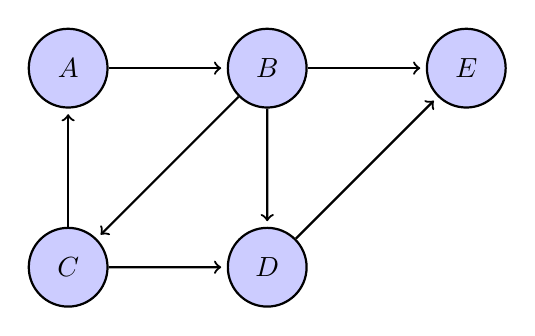
\begin{tikzpicture}[thick,scale=0.8,->,shorten >=2pt]
    \node[main node] (A) {$A$};
    \node[main node] (B) [right= 1.5cm of A]  {$B$};
    \node[main node] (C) [below= 1.5cm of A] {$C$};
    \node[main node] (D) [below= 1.5cm of B] {$D$};
    \node[main node] (E) [right =1.5cm of B] {$E$};

    \path[draw,thick]
    (A) edge node {} (B)
    (B) edge node {} (C)
    (C) edge node {} (A)
    (B) edge node {} (D)
    (C) edge node {} (D)
    (B) edge node {} (E)
    (D) edge node {} (E);
  \end{tikzpicture}
\end{center}
  }
\end{document}
